\chapter{Stand der Technik}
\section{Getränkemischmaschine}
Ziel dieser Arbeit ist die Implementierung einer Sprachsteuerung für eine Getränkemischmaschine. Die Getränkemischmaschine wurde bereits in einem vorangegangenen Projekt erstellt \cite{mischmaschine}. In diesem Abschnitt wird darauf eingegangen, um was für eine Art von Maschine es sich dabei handelt und es werden ihre Funktionsweise und ihr Aufbau beschrieben.\\\\
Das Mischen von Getränken bzw. Flüssigkeiten ist der Anwendungsfall für den die Maschine konzipiert wurde. Dazu besitzt die Mischmaschine fünf Behälter zu je einem Liter. Jedem Behälter ist eine Pumpe zugeordnet, die separat angesteuert werden kann und dafür sorgt, dass die Flüssigkeit aus dem Behälter zur Getränkeausgabe gelangt. Kurz vor dem Ausgang werden die Schläuche der Behälter zusammengeführt, wodurch letztlich die Mischung der verschiedenen Getränke erzielt wird. Sogenannte \glqq{}Rückschlagventile\grqq{} sorgen dafür, dass ein Zurückfließen der Getränkemischung in die Behälter verhindert wird.\\\\
Zur Steuerung der Maschine durch einen Benutzer befinden sich an der Vorderseite zwei Knöpfe und ein Touch-Display. Einer der Knöpfe dient dem Anschalten der Maschine und ein weiterer der Ausgabe des Getränks. Über das Touch-Display kann der Benutzer die Mischung seiner Getränke konfigurieren und die Maschine administrieren.\\\\
\begin{figure}[H]
    \centering
    \fbox{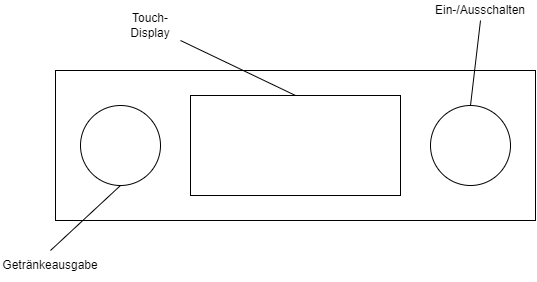
\includegraphics[width=0.8\textwidth]{img/Bilder_Kapitel_2/Bedienungsschnittstelle_Mischmaschine.png}}
    \caption{Schematischer Aufbau der Bedienungsschnittstelle}
    \label{fig:bedienungsschnittstelle_mischmaschine}
\end{figure}
\noindent
Abbildung \ref{fig:bedienungsschnittstelle_mischmaschine} stellt den schematischen Aufbau der Bedienungsschnittstelle der Getränkemischmaschine für ein besseres Verständnis dar.\\\\
Die technische Umsetzung basiert auf der Kommunikation zwischen dem Touch-Display und einem, in der Getränkemischmaschine verbauten, Arduino, der anhand der Daten von der Benutzereingabe, die Pumpen steuert. Beim Drücken des Startknopfes werden das Display und der Arduino mit Strom versorgt, sodass sowohl das Display als auch der Arduino starten und mit der Ausführung des benutzerdefinierten Quelltextes beginnen. Auf dem Bediendisplay findet sich fünf Schieberegler - ein Schieberegler je Behälter - mit denen der Benutzer die Zusammensetzung seines Mischgetränks aus den fünf Behältern konfigurieren kann. Beim Drücken eines in der \ac{UI} des Displays dargestellten Knopfes werden die Werte der Schieberegler an den Arduino übertragen. Dieser rechnet die Prozentwerte der Schieberegler in Durchsatzraten für die Pumpen um. Wird anschließend der Knopf für die Getränkeausgabe gedrückt gehalten steuert der Arduino die Pumpen mit ihrer jeweiligen Durchsatzrate an und der Anwender bekommt sein Mischgetränk ausgegeben.
\section{Hardware}
\section{Sprachverarbeitung}
Im Zuge des technologischen Fortschritts nutzen die Menschen heutzutage zunehmend Sprachassistenten für verschiedene Aufgaben. 
Einer der Hauptvorteile der Sprachsteuerung ist die Bequemlichkeit und Geschwindigkeit, mit der Aufgaben erledigt werden können, ohne dass man tippen oder mit der Maus klicken muss. 
Sprachassistenten nutzen die Verarbeitung natürlicher Sprache, um Befehle zu erkennen und zu verstehen, die der Nutzer laut ausspricht.\\\\
Die Verarbeitung natürlicher Sprache - \ac{NLP} - ist eine wichtige Technologie, die es Computern ermöglicht, die von Menschen verwendete natürliche Sprache zu verstehen. 
Diese Technologie ermöglicht es Computern, menschliche Sprache zu erkennen und zu interpretieren und Text und Sprache in natürlicher Sprache zu erzeugen. 
Im Bereich der Sprachsteuerung spielt \ac{NLP} eine Schlüsselrolle bei der Erkennung von Sprache und dem Verstehen von Befehlen, die der Benutzer laut ausspricht. 
Es wird verwendet, um die Sprache des Benutzers in Text umzuwandeln, den ein Computer verstehen und verarbeiten kann.
Um dies zu erreichen, verwendet \ac{NLP} eine Vielzahl von Techniken und Technologien, darunter maschinelles Lernen, Tonanalyse, syntaktische Analyse und mehr. \cite{jurafsky_speech_2009}\\\\
Im Rahmen dieses Projekts erfordert die Implementierung der Sprachsteuerung einer Getränkemischmaschine die Verarbeitung natürlicher Sprache, damit die Maschine Befehle verstehen kann, die der Benutzer laut ausspricht. 
Dieses Projekt ähnelt einem Chatbot, bei dem der Benutzer eine Frage stellen oder einen Befehl geben kann und der Chatbot führt die entsprechende Aktion aus. 
Die Verarbeitung natürlicher Sprache ist für die Entwicklung eines solchen Sprachsteuerungssystems unerlässlich und ermöglicht es der Maschine, Befehle in natürlicher Sprache zu verstehen und auszuführen.\\\\
Eine der wichtigsten Komponenten der Verarbeitung natürlicher Sprache ist die Spracherkennung und das Syntaxanalyseverfahren. 
Bei der Spracherkennung kommen Deep-Learning-Techniken zum Einsatz, die es einem Computer ermöglichen, Sprachlaute zu erkennen und in Text zu übersetzen. 
Anschließend wird das Syntaxanalyseverfahren verwendet, um die Satzstruktur zu bestimmen und Schlüsselwörter und -sätze hervorzuheben, die zur Bestimmung des Benutzerbefehls verwendet werden können.
Auch die Tonwertanalyse ist ein wichtiger Bestandteil der Verarbeitung natürlicher Sprache. 
Mit Hilfe der Tonalitätsanalyse lässt sich die emotionale Färbung des Textes bestimmen, was für die Ermittlung der Absicht des Nutzers nützlich sein kann. 
Da die Tonwertanalyse im Rahmen dieser Arbeit nicht relevant ist, wird sie nicht weiter erörtert.\\\\
Darüber hinaus werden grammatik- und regelbasierte Technologien zur Verarbeitung natürlicher Sprache eingesetzt. 
Diese Technologien werden eingesetzt, um die korrekte Struktur des Benutzerbefehls zu bestimmen und Schlüsselwörter hervorzuheben, die zur Durchführung von Aktionen verwendet werden können. 
Außerdem werden Techniken des maschinellen Lernens eingesetzt, damit der Computer aus früheren Befehlen und Aktionen \glqq{}lernen\grqq{} kann, was die Genauigkeit der Erkennung von Benutzerbefehlen verbessert.\\\\
Daher ist der Einsatz von Technologien zur Verarbeitung natürlicher Sprache für das Projekt der Sprachmischmaschine unerlässlich. 
Die Verarbeitung natürlicher Sprache wird es der Maschine ermöglichen, die Befehle zu verstehen und zu verarbeiten, die der Benutzer laut ausspricht und die entsprechenden Aktionen durchzuführen.
\subsection{Verarbeitung natürlicher Sprache}
Die Verarbeitung natürlicher Sprache ist ein Forschungsbereich der Informatik und der \ac{KI}, der sich mit der Verarbeitung natürlicher Sprache befasst. 
Bei der Verarbeitung geht es in der Regel darum, natürliche Sprache in Daten zu übersetzen, die ein Computer nutzen kann, um Informationen über die Welt um ihn herum zu erhalten.\\\\
Die \ac{NLP}-Pipeline, die zur Erstellung eines Dialogsystems erforderlich ist, erfordert vier Arten der Verarbeitung sowie eine Datenbank zur Speicherung vergangener Äußerungen und Antworten. 
Jeder dieser Schritte kann einen oder mehrere Verarbeitungsalgorithmen enthalten, die parallel oder sequentiell arbeiten \cite{lane_natural_2019}:
\begin{itemize}
    \item Syntaktische Zergliederung - Extraktion von Merkmalen (strukturierte numerische Daten) aus natürlichem Text.
    \item Analyse - Erstellen und Kombinieren von Items, um Indikatoren für den Ton, die grammatikalische Korrektheit und die Semantik des Textes zu erhalten.
    \item Generierung - Generierung möglicher Antworten mit Hilfe von Mustern, Suchwerkzeugen oder Sprachmodellen.
    \item Ausführung - bereitet Aussagen vor, die auf der Geschichte und dem Zweck des Gesprächs basieren und wählt eine Folgeantwort.
\end{itemize}
\begin{figure}[H]
    \centering
    \fbox{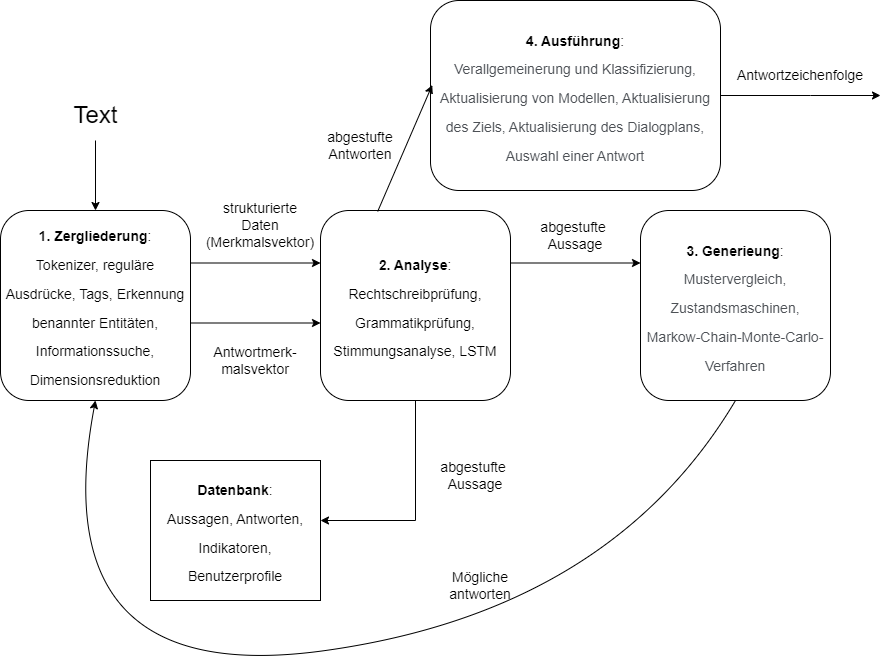
\includegraphics[width=0.8\textwidth]{Bilder_Kapitel_2/Chat-Bot-Pipeline.png}}
    \caption{Rekurrente Chat-Bot-Pipeline}
    \label{figure:Chat-Bot-Pipeline}
\end{figure}
\noindent
Die meisten Chatbots enthalten Elemente aus allen fünf Teilsystemen (die vier Verarbeitungsstufen sowie die Datenbank). 
Viele Anwendungen erfordern jedoch nur einfache Algorithmen, um viele dieser Schritte auszuführen. 
Ein Chatbot oder virtueller Assistent für Verbraucher wie Alexa oder Allo ist in der Regel so konzipiert, dass er äußerst sachkundig und leistungsfähig ist. 
Die Logik, die zur Beantwortung von Anfragen verwendet wird, ist jedoch oft oberflächlich und besteht aus einer Reihe von Codephrasen, die mit einer einzigen if-then-Entscheidungsverzweigung zur gleichen Antwort führen. 
Alexa (und die zugrundeliegende Lex-Engine) verhält sich wie ein einschichtiger, flacher Baum von Operatoren (if, elif, elif...). 
Andererseits stützt sich die Google Translate-Pipeline (oder jedes ähnliche maschinelle Übersetzungssystem) auf eine mehrstufige Hierarchie von Merkmalsextraktoren, Entscheidungsbäumen und Wissensgraphen, die Fragmente von Wissen über die Welt miteinander verbinden.\\\\
Alle \ac{NLP}-Merkmale müssen gut funktionieren, damit das Dialogsystem richtig funktioniert:
\begin{itemize}
    \item Merkmalsextraktion (normalerweise zur Erstellung eines Vektorraummodells).
    \item Informationssuche zur Beantwortung von Sachfragen.
    \item Semantische Suche, um Informationen aus zuvor aufgezeichneten natürlichsprachlichen Texten oder Dialogen zu assimilieren.
    \item Generierung von natürlicher Sprache, um neue sinnvolle Aussagen zu verfassen.
\end{itemize}
\subsection{Tokenisierung von Wörtern}
Eine der wichtigsten Aufgaben der Verarbeitung natürlicher Sprache ist die Tokenisierung, d. h. die Zerlegung von Text in einzelne Wörter oder Phrasen, die so genannten Token. 
Dieser Prozess ist ein wichtiger Bestandteil der Verarbeitung natürlicher Sprache, da er es Programmen und Algorithmen ermöglicht, Texte anhand ihrer Bestandteile zu verstehen und zu analysieren. 
Die Tokenisierung ist für die Verarbeitung natürlicher Sprache von entscheidender Bedeutung, da sie es Programmen ermöglicht, Schlüsselwörter, Phrasen und semantische Einheiten in einem Text hervorzuheben. 
Die Tokenisierung kann auch dazu verwendet werden, nicht benötigte Textelemente wie Satzzeichen, Leerzeichen und andere Zeichen, die keine Bedeutung haben, zu entfernen. 
Dadurch können Programme und Algorithmen effizienter und genauer arbeiten und die Wahrscheinlichkeit von Fehlern und falscher Textverarbeitung verringern.\\\\
Im \ac{NLP} ist die Tokenisierung eine besondere Art der Segmentierung von Dokumenten. 
Bei der Segmentierung wird der Text in kleinere Abschnitte (Segmente) mit engerem Informationsgehalt unterteilt. 
Die Segmentierung kann die Aufteilung eines Dokuments in Absätze, in Sätze, in Phrasen und in Token (Wörter) sowie Satzzeichen umfassen. 
Ein Tokenizer kann mit einem Scanner im Kompilierungsprozess verglichen werden. 
Token sind in diesem Fall die Endpunkte von kontextfreien Grammatiken - \ac{CFG} - zur Analyse von Programmiersprachen-Terminalen.\\\\
Die Tokenisierung ist der erste Schritt in der \ac{NLP}-Pipeline und kann daher den Rest der Pipeline stark beeinflussen. 
Der Tokenizer zerlegt unstrukturierte Daten, d. h. natürlichsprachliche Texte, in Informationseinheiten, die als einzelne Elemente gezählt werden können. 
Die so gezählte Anzahl von Token-Vorkommen in einem Dokument kann direkt als Vektor verwendet werden, der dieses Dokument repräsentiert. 
Ein solcher Ansatz ermöglicht es, aus einer unstrukturierten Zeichenfolge (einem Textdokument) unmittelbar eine für das maschinelle Lernen geeignete numerische Datenstruktur zu gewinnen. 
Diese Werte können den Computer direkt dazu veranlassen, nützliche Aktionen durchzuführen und Reaktionen zu erzeugen.\\\\
Die einfachste Art, einen Satz zu tokenisieren, ist die Verwendung von Leerzeichen als Worttrenner in Zeichenketten. 
Dies ist jedoch nicht optimal, denn wenn ein Satz z. B. ein Satzzeichen enthält, wird es von einem der Tokenisierer erfasst. 
Optimierte Tokenizer sind in mehreren Python-Bibliotheken implementiert, die jeweils ihre eigenen Vor- und Nachteile haben: spaCy, Stanford CoreNLP und \ac{NLTK}. 
\ac{NLTK} und StanfordCoreNLP sind die am längsten bestehenden und am häufigsten verwendeten Bibliotheken zum Vergleich von \ac{NLP}-Algorithmen in wissenschaftlichen Artikeln. 
Obwohl die StanfordCoreNLP-Bibliothek eine Python-API hat, basiert sie auf dem Java 8 CoreNLP-Anwendungsteil, der separat installiert und konfiguriert werden muss. 
Daher wurde in dieser Arbeit der \ac{NLTK}-Tokenizer verwendet.\\\\
Ein wichtiges Konzept im Tokenisierungsprozess sind N-Gramme. 
Ein N-Gramm ist eine Sequenz mit bis zu n Elementen, die aus einer Sequenz dieser Elemente, in der Regel einer Zeichenkette, extrahiert wurden. 
Im Allgemeinen können die Elemente eines N-Gramms Buchstaben, Silben, Wörter oder sogar Symbole sein. 
N-Gramme sind notwendig, weil bei der Konvertierung einer Menge von Wörtern in einen Vektor eine Folge von Token einen Großteil der Bedeutung verliert, die in der Reihenfolge dieser Wörter verkapselt ist. 
Wenn das Token-Konzept auf Mehrwort-Token, N-Gramme, ausgedehnt wird, kann die \ac{NLP}-Pipeline einen erheblichen Teil der Bedeutung, die in der Wortfolge dieser Äußerungen enthalten ist, beibehalten. 
So bleibt beispielsweise das Wort \glqq{}kein\grqq{}, das die Bedeutung umkehrt, neben den benachbarten Wörtern stehen, wo es hingehört. 
Ohne N-Gramm-Tokenisierung würde ein solches Wort an verschiedenen Positionen herumhängen und seine Bedeutung würde mit dem gesamten Satz oder Dokument assoziiert werden, anstatt mit benachbarten Wörtern. 
Das Bigramm \glqq{}war nicht\grqq{} behält viel mehr Bedeutung der einzelnen Wörter \glqq{}war\grqq{} und \glqq{}nicht\grqq{} als die entsprechenden Singlegramme im Multigrammvektor. 
Durch die Verknüpfung eines Wortes mit seinen Nachbarn in einem Förderband kann ein Teil seines Kontexts erhalten bleiben. 
N-Gramme sind also ein Instrument zur Speicherung von Kontextinformationen, während die Daten die Pipeline durchlaufen.\\\\
Die Größe des Vokabulars spielt eine wichtige Rolle für die Leistung der \ac{NLP}-Pipeline. 
Die Größe des Wörterbuchs bestimmt die Größe der Trainingsstichprobe, die benötigt wird, um eine Überanpassung an ein bestimmtes Wort oder eine bestimmte Phrase zu vermeiden und die Größe der Trainingsmenge bestimmt die Kosten der Verarbeitung. 
Eine Technik zur Verringerung der Größe des Wörterbuchs besteht darin, Token, die ähnliche Dinge bedeuten, in einer einzigen normalisierten Form zusammenzufassen. 
Eine solche Technik reduziert die Anzahl der gespeicherten Token und verbessert die Verbindungen zwischen den Bedeutungen von Phrasen mit unterschiedlicher \glqq{}Schreibweise\grqq{} der Tokens und verringert die Wahrscheinlichkeit des Überlernens. 
Eine der Normalisierungsmöglichkeiten ist die Groß- und Kleinschreibung - die Kombination mehrerer Schreibweisen eines Wortes, die sich nur in der Groß- und Kleinschreibung unterscheiden. 
In diesem Fall wird die Groß-/Kleinschreibung ignoriert und zwei identische Wörter, von denen eines groß und das andere klein geschrieben wird, werden als dasselbe Token behandelt.\\\\
Ein weiterer wichtiger Schritt bei der Tokenisierung von Texten ist die Entfernung von Stoppwörtern, um den Umfang des Wörterbuchs zu verringern. 
Stoppwörter sind in jeder Sprache gebräuchliche Wörter, die sehr häufig vorkommen, aber sehr viel weniger aussagekräftige Informationen über die Bedeutung eines Satzes enthalten (z. B. a, an, the, this, of, on im Englischen oder der, die, das, diese im Deutschen). 
Stoppwörter können jedoch nützliche Informationen enthalten, so dass man sie nicht immer verwerfen sollte. 
Das \ac{NLTK}-Paket für Python enthält derzeit die umfassendste Liste kanonischer Stoppwörter in verschiedenen Sprachen.\\\\
Eine weitere gängige Methode der Normalisierung ist die Beseitigung kleiner semantischer Unterschiede im Zusammenhang mit Pluralendungen und Possessivendungen von Wörtern oder sogar unterschiedlichen Verbformen. 
Diese Methode der Normalisierung, bei der ein gemeinsamer Wortstamm für verschiedene Wortformen gefunden wird, wird als Stemming bezeichnet. 
Der gemeinsame Wortstamm von \glqq{}Gehäuse\grqq{} und \glqq{}Haus\grqq{} ist zum Beispiel \glqq{}Haus\grqq{}.
 Beim Stemming werden Suffixe von Wörtern entfernt, um Wörter mit ähnlicher Bedeutung unter einem gemeinsamen Stamm zu gruppieren. 
 Der Wortstamm muss nicht unbedingt ein gültiges Wort sein, sondern kann auch nur ein Token oder eine Bezeichnung sein, das mehrere mögliche Schreibweisen repräsentiert. 
 Einer der Hauptvorteile des Stemming besteht darin, die Anzahl der Wörter zu verringern, deren Bedeutung das Sprachmodell im Auge behalten muss. 
 Durch diese Methode wird die Größe des Wörterbuchs reduziert, wodurch der Verlust nützlicher Informationen und Bedeutungen so weit wie möglich begrenzt wird. 
 Das Stemming spielt eine wichtige Rolle bei der Suche nach Schlüsselwörtern oder Informationen. 
Zwei der bekanntesten Algorithmen sind Porter's Stemmer und Snowball.\\\\
Mit Informationen über die Beziehungen zwischen den Bedeutungen verschiedener Wörter ist es möglich, mehrere Wörter miteinander zu verknüpfen, auch wenn ihre Schreibweise sehr unterschiedlich ist. 
Eine solche erweiterte Normalisierung eines Wortes auf seine semantische Wurzel - ein Lemma - wird Lemmatisierung genannt. 
Die Lemmatisierung ist potenziell eine viel genauere Art der Normalisierung als das Stemming oder die Groß- und Kleinschreibung, da sie die Bedeutung des Wortes berücksichtigt. 
Der Lemmatisierer verwendet eine Wissensbasis von Synonymen und Wortendungen, um nur eng verwandte Wörter zu einem Token zu kombinieren. 
In Python kann die Lemmatisierung mit dem \ac{NLTK}-Paket implementiert werden, das den \textit{WordNetLemmatizer} enthält.\\\\
Wie bereits gezeigt wurde, ist die Tokenisierung der Prozess der Zerlegung von Text in einzelne Wörter oder Token. 
Für viele Anwendungen der Verarbeitung natürlicher Sprache ist jedoch nicht nur wichtig, welche Wörter im Text enthalten sind, sondern man muss auch in der Lage sein, diese Wörter als Zahlen darzustellen. 
Dadurch wird es möglich, maschinelles Lernen und andere Algorithmen, die mit Zahlen arbeiten, zur Textverarbeitung einzusetzen. 
Bei der Verarbeitung natürlicher Sprache wird dazu die Wortvektorisierung verwendet.
\subsection{Vektoren von Wörtern}
\subsection{Syntaktische Analyse}
\subsection{Ansätze für die Erstellung eines Chatbots}\label{sec:ansaetze_erstellung_chatbots}
Derzeit gibt es vier Hauptansätze für die Erstellung eines Chatbots \cite{lane_natural_2019}:
\begin{itemize}
    \item Musterabgleich: Musterabgleich und Antwortvorlagen (vorgefertigte Antworten)
    \item Grounding: logische Wissensgraphen und das Ziehen von Schlussfolgerungen aus diesen basierend auf diesen Graphen
    \item Suche: Abrufen von Text
    \item Generierungsmethoden: Statistik und maschinelles Lernen
\end{itemize}
Die vier grundlegenden Ansätze zur Erstellung von Chatbots lassen sich kombinieren, was zu benutzerfreundlicheren Chatbots führt. 
Eine Vielzahl von Anwendungen nutzen alle vier grundlegenden Methoden. 
Hybride Chatbots unterscheiden sich hauptsächlich darin, wie genau sie diese Ansätze kombinieren und wie viel Gewicht auf jeden einzelnen Ansatz gelegt wird.
\subsubsection{Musterabgleich}
Bei den ersten Chatbots basierte die Antwort auf die Nachricht eines Benutzers auf einem Mustervergleich. 
Diese Chatbots suchen nach Mustern im eingehenden Text und geben eine feste (gemusterte) Antwort, wenn eine Übereinstimmung gefunden wird \cite{woudenberg_chatbot_2014}.\\\\
Solche rudimentären Dialogsysteme sind vor allem in automatisierten Benutzerunterstützungssystemen mit interaktiven Sprachmenüs nützlich, wo es möglich ist, das Gespräch an einen Menschen weiterzuleiten, wenn der Chatbot keine Antwortmuster mehr hat.\\\\
Da es viele \ac{NLP}-Dienstprogramme in Python-Paketen gibt, ist es möglich, komplexere Chatbots auf der Grundlage von Mustervergleichen zu erstellen, indem man die Bot-Logik nach und nach direkt in Python mit regulären Ausdrücken und Suchmustern aufbaut.\\\\
1995 machte sich Richard Wallace daran, einen allgemeinen Rahmen für die Erstellung von Chatbots auf der Grundlage des Pattern-Matching-Ansatzes zu schaffen. Zwischen 1995 und 2002 schuf seine Entwicklergemeinschaft die \ac{AIML} zur Beschreibung von Mustern und Chatbot-Antworten.\\\\
\ac{AIML} ist eine deklarative Sprache, die auf dem \ac{XML}-Standard basiert, der die Sprachkonstrukte und Datenstrukturen einschränkt, die im Bot verwendet werden dürfen. \cite{noauthor_aiml_nodate}
Ein Chatbot, der auf \ac{AIML} basiert, sieht folgendermaßen aus:
\begin{figure}[H]
    \centering
    \fbox{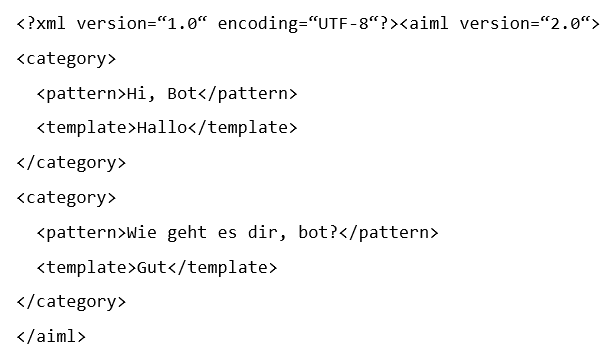
\includegraphics[width=0.8\textwidth]{Bilder_Kapitel_2/aiml_bot.png}}
    \caption{\label{figure:Aiml_Bot}\ac{AIML} Chatbot}
\end{figure}
\noindent
Eine der Einschränkungen von \ac{AIML} ist die Art der Muster, die abgeglichen werden können und auf die reagiert wird. 
Der \ac{AIML}-Kern (Pattern Matching Engine) reagiert nur auf Eingabetext, der einem vom Entwickler manuell vorgegebenen Muster entspricht. 
Unscharfe Suchanfragen, Smileys, Satzzeichen, Tippfehler oder falsch geschriebene Wörter sind nicht erlaubt, es findet kein automatischer Abgleich statt. 
In \ac{AIML} müssen alle Synonyme manuell einzeln beschrieben werden.
\subsubsection{Grounding}
Die Grounding-Methode ist ein Ansatz zur Erstellung eines Chatbots auf der Grundlage logischer Wissensgraphen und der Durchführung von Schlussfolgerungen auf der Grundlage dieser Graphen. \cite{diana_conversational_2011}
Sie wird verwendet, um natürliche Sprache zu verarbeiten und sie dem Verständnis des Bots zuzuordnen. Das Wesentliche an der Grounding-Methode ist, dass der Chatbot nicht nur die Textnachrichten, sondern auch den Kontext und die Umgebung verarbeitet, um Anfragen besser zu verstehen und zu beantworten. 
Durch die Extraktion von Informationen wird ein Netz von Verbindungen oder Fakten geschaffen. Dieses Netz logischer Verbindungen zwischen Entitäten - ein Graph oder eine Wissensbasis - kann die Grundlage für die Antworten des Chatbots bilden.\\\\
Ein Beispiel für eine Grounding-Methode ist die Verwendung eines Wissensgraphen zur Beschreibung der Umgebung. 
Ein Wissensgraph enthält Informationen über die Objekte, mit denen der Bot interagieren kann und die Beziehungen zwischen ihnen. 
Ein Wissensgraph könnte zum Beispiel Informationen über ein Glas auf einem Tisch und das darin befindliche Wasser enthalten. 
Wenn ein Benutzer eine Frage stellt, verwendet der Chatbot den Wissensgraphen, um den Kontext der Anfrage zu verstehen und die am besten geeignete Antwort abzuleiten. 
Wenn ein Benutzer zum Beispiel fragt: \glqq{}Wie hoch ist die Temperatur des Wassers in dem Glas auf dem Tisch?\grqq{}, kann der Chatbot Informationen aus dem Wissensgraphen verwenden, um die Frage zu beantworten.\\\\
Ein solcher Wissensgraph kann abgeleitet werden, um Fragen über die in dieser Wissensbasis enthaltene Welt zu beantworten und anschließend können auf der Grundlage der logischen Antworten die Werte der in den Antworten enthaltenen Template-Variablen ausgefüllt werden, um natürlichsprachliche Antworten zu erstellen. 
Ursprünglich wurden auf diese Weise Systeme zur Beantwortung von Fragen eingerichtet, wie z. B. der Watson-Bot von IBM (heutzutage wird für ähnliche Systeme jedoch die Informationssuchemethode verwendet). 
Der Wissensgraph stellt eine Art \glqq{}Erdung\grqq{} des Chatbots in der realen Welt dar.\\\\
Die Erstellung von Chatbots auf der Grundlage von \glqq{}Grounding\grqq{} eignet sich hervorragend für Chatbots, die Fragen generieren, bei denen das zur Beantwortung einer Frage erforderliche Wissen in einer umfangreichen Wissensbasis enthalten ist, die aus einer offenen Datenbank (z. B. Wikidata, Open Mind Common Sense oder DBpedia) bezogen werden kann.\\\\
Einer der Hauptvorteile der Grounding-Methode besteht darin, dass sie sich an ein sich veränderndes Umfeld anpassen kann. 
Wenn der Benutzer zum Beispiel ein Glas Wasser von einem Tisch auf einen anderen stellt, wird der Wissensgraph automatisch aktualisiert, um diese Änderung widerzuspiegeln.\\\\
Die Grounding-Methode hat jedoch auch ihre Grenzen. 
So kann es vorkommen, dass bei der Verarbeitung großer Informationsmengen Zusammenhänge nicht berücksichtigt werden und dem Bot möglicherweise verborgen bleiben.\\\\
Insgesamt ist die Grounding-Methode ein effektiver Ansatz zur Erstellung wissensbasierter Chatbots. 
Sie ermöglicht es dem Bot, Benutzeranfragen besser zu verstehen und eine genauere Antwort zu geben.
\subsubsection{Suche}
Die Informationssuchemethode ist eine der Methoden zum Aufbau von Chatbots, die auf der Extraktion von Informationen aus einer großen Menge von Textinformationen basiert. 
Die Hauptidee der Informationssuchemethode ist die Analyse des Eingabetextes (Benutzeranfrage), die Auswahl von Schlüsselwörtern und Phrasen daraus und die anschließende Suche nach den relevantesten Informationen in der Wissensdatenbank oder in offenen Quellen. \cite{diana_conversational_2011}\\\\
Die Wissensbasis kann auch eine Art \glqq{}Gesprächsprotokoll\grqq{} sein, in Form von Aussage-Antwort-Paaren. 
Dabei sucht der Bot nach früheren Aussagen in den Protokollen früherer Unterhaltungen. 
Der Bot kann nicht nur in den Protokollen seiner eigenen Gespräche suchen, sondern auch in beliebigen Transkripten von Gesprächen zwischen Menschen, Gesprächen zwischen Menschen und Bots oder sogar Gesprächen zwischen Bots.
Aber wie immer gilt: je besser die Eingabedaten, desto besser das Ergebnis. 
Daher ist es notwendig, die Datenbank früherer Gespräche sorgfältig zu säubern und zu organisieren, damit der Bot nach einem qualitativ hochwertigen Gespräch sucht und es dann imitiert.\\\\
Für die Umsetzung der Informationssuchemethode werden verschiedene Algorithmen und Techniken verwendet, z. B. Indizierung und Schlagwortsuche, Kontextsuche, Textanalyse mit Hilfe von maschinellen Lernverfahren usw. 
Die Informationssuchemethode kann in Python mit verschiedenen Bibliotheken und Tools wie \ac{NLTK}, Scikit-learn und Gensim implementiert werden.\\\\
Einer der ersten Schritte bei der Implementierung einer Informationssuchemethode in Python ist die Vorbereitung der Daten. 
Dies erfordert Tokenisierung, Lemmatisierung und die Entfernung von Stopp-Wörtern. 
Als nächstes muss ein Index auf der Grundlage von Schlüsselwörtern erstellt werden. 
Der Index kann auf der Grundlage von Bag-of-Words oder \ac{TF} und \ac{IDF} (TF-IDF-Modelle) erstellt werden. 
Sobald der Index erstellt ist, kann eine Stichwortsuche durchgeführt werden. 
Dazu muss die Benutzeranfrage in einen Vektor umgewandelt und mit den Dokumentvektoren im Index verglichen werden. 
Dies kann mit Hilfe der Scikit-learn-Bibliothek erfolgen \cite{scikit-learn}.
Sobald die relevantesten Dokumente gefunden wurden, können sie in eine Rangfolge gebracht und als Antwort auf die Benutzeranfrage angezeigt werden.\\\\
Der Vorteil der Informationssuchemethode besteht darin, dass sie ein schnelles und genaues Auffinden der gewünschten Informationen ermöglicht, insbesondere wenn die Wissensbasis gut strukturiert ist und genügend Informationen enthält. 
Ein Nachteil dieser Methode ist jedoch, dass sie den Kontext der Anfrage nicht berücksichtigt und nicht immer eine vollständige und genaue Antwort auf die Frage des Nutzers liefert. 
Wenn die Aussage semantisch mit der vom Bot zu beantwortenden übereinstimmt, ist es möglich, die Antwort wortwörtlich und ohne Änderungen wiederzuverwenden. 
Aber selbst wenn die Datenbank alle möglichen Benutzeräußerungen enthält, wird der Bot die Persönlichkeiten der Personen widerspiegeln, die diese Äußerungen machen. 
Wenn die Antworten konsistent sind und von einer Vielzahl von Personen stammen, ist das gut. 
Problematisch wird es jedoch, wenn die Äußerung, auf die der Bot reagieren soll, vom Gesamtkontext des jeweiligen Gesprächs oder von den Umständen in der Umgebung abhängt, die sich seit der Erstellung des Dialogkorpus geändert haben können.\\\\
Beispielsweise sollte der Bot auf die Frage \glqq{}Wie spät ist es?\grqq{} nicht die von der Person gegebene Antwort, sondern die am besten geeignete Aussage aus der Datenbank verwenden. 
Diese Antwort funktioniert nur, wenn die Zeit, zu der die Frage gestellt wurde, mit der Zeit übereinstimmt, zu der die passende Äußerung aus der Datenbank aufgezeichnet wurde. 
Neben dem natürlichsprachlichen Text der Äußerung müssen auch ähnliche Informationen über die Zeit - der Kontext (Zustand) - erfasst und verglichen werden. 
Sie spielt vor allem dann eine wichtige Rolle, wenn die Semantik der Äußerung auf eine aktive Veränderung des im Kontext (Wissensbasis des Chatbots) erfassten Zustands hinweist.\\\\
Um den Zustand (Kontext) in einem Chatbot auf der Grundlage der Informationssuche zu berücksichtigen, kann etwas Ähnliches für einen Chatbot mit Musterabgleich durchgeführt werden, da die Auflistung einer Liste von Benutzeraussagen nur eine andere Art ist, ein Muster zu beschreiben. 
Dies auch ist der Ansatz von Amazon Lex \cite{amazon_lex} und Google Dialogflow \cite{dialogflow_chawla}. 
Anstatt ein starres Muster zu beschreiben, um den Befehl des Benutzers zu erfassen, können der Dialogflow-Engine einfach ein paar Beispiele geliefert werden. 
So wie jedes Muster im Chatbot auf der Grundlage der Musterzuordnung einem Zustand zugeordnet wurde, muss auch hier nur die Aussage-Antwort-Beispielpaare mit dem genannten Zustand verknüpft werden.\\\\
Der suchbasierte Chatbot indiziert also den Korpus der Dialoge, so dass er leicht frühere Aussagen finden kann, die derjenigen ähnlich sind, auf die er antworten muss und antwortet dann mit einer der passenden Aussagen aus dem Korpus, die er sich \glqq{}gemerkt\grqq{} und für eine schnelle Suche indiziert hat. 
Im Allgemeinen ist die Methode der Informationssuche eine der gängigsten und beliebtesten Methoden zum Aufbau von Chatbots, die in verschiedenen Bereichen wie Wirtschaft, Medizin, Tourismus und vielen anderen eingesetzt werden.
\subsubsection{Generierungsmethoden}
Generierungsmethoden sind einer der wichtigsten Ansätze bei der Entwicklung von Chatbots auf der Grundlage künstlicher Intelligenz. 
Sie ermöglichen es Chatbots, Textantworten auf der Grundlage der Analyse der eingehenden Nachricht und des Kontextes des Dialogs zu generieren. 
Die folgenden Generierungsmodelle sind nützlich, um einen kreativen Chatbot zu erstellen, der Dinge sagen kann, die noch niemand zuvor gesagt hat:
\begin{itemize}
    \item Sequenz-zu-Sequenz-Konvertierungsmodelle: Modelle, die darauf trainiert sind, Antworten auf der Grundlage von Eingabesequenzen zu generieren;
    \item \ac{RBM}: Markov-Ketten, die so trainiert werden, dass sie die \glqq{}Energie\grqq{}-Funktion minimieren \cite{chatbot_development_sharma};
    \item \ac{GAN}: statistische Modelle, die darauf trainiert sind, einen Experten, der die Qualität eines Gesprächs bewertet, zu täuschen. \cite{li_adversarial_2017}
\end{itemize}
Die Vorteile des Einsatzes der Generierungsmethoden:
\begin{itemize}
    \item Flexibilität: Generative Methoden können für eine breite Palette von Aufgaben eingesetzt werden, einschließlich Texterstellung, Sprachübersetzung, Verarbeitung natürlicher Sprache und mehr.
    \item Automatisierung: Generative Methoden können auf großen Datensätzen trainiert werden, wodurch die Erstellung von Inhalten automatisiert werden kann.
    \item Qualität: Generative Methoden zeigen eine hohe Qualität bei der Textgenerierung, Sprachübersetzung und anderen Aufgaben der natürlichen Sprachverarbeitung, wenn sie auf einem ausreichend großen Datensatz trainiert werden.
    \item Schnelligkeit: Generative Methoden können schneller arbeiten als Menschen, was die Erstellung von Inhalten mit großer Geschwindigkeit ermöglicht.
\end{itemize}
Die Nachteile der generativen Methoden:
\begin{itemize}
    \item Große Datenmengen für das Training: Generative Methoden benötigen große Datenmengen für das Training, was bei einigen Aufgaben schwierig sein kann, insbesondere wenn nur ein kleiner Datensatz zur Verfügung steht.
    \item Sicherheitsrisiken: Generative Methoden können Inhalte erzeugen, die möglicherweise falsch, unvollständig oder irreführend sind. Dies kann zu Sicherheitsrisiken führen, wenn der generierte Inhalt für wichtige Entscheidungen verwendet wird.
    \item Unterstützungsbedarf: Generative Methoden können erhebliche Unterstützung benötigen, um effektiv zu sein. Dies kann die Modellabstimmung, die Auswahl optimaler Parameter und die Optimierung der Modellleistung auf einer bestimmten Hardwarekonfiguration umfassen.
    \item Modellbeschränkungen: Generative Methoden können Beschränkungen hinsichtlich der Arten von Inhalten haben, die sie erzeugen können, insbesondere wenn sie nur auf bestimmte Datentypen trainiert wurden.
\end{itemize}
Eine der beliebtesten Methoden zur Texterstellung ist die sequence-to-sequence-Methode (seq2seq). 
Die seq2seq-Methode basiert auf \ac{RNN}, die die Simulation von Datenfolgen ermöglichen. 
Sie besteht aus zwei Hauptteilen: einem Encoder und einem Decoder. 
Ein Encoder empfängt eine Wortfolge und baut daraus einen Kontextvektor auf, der Informationen über die Eingabedaten enthält. 
Der Decoder erhält diesen Vektor als Eingabe und beginnt mit der Generierung einer Folge von Antwortnachrichten, wobei er schrittweise den Kontext und die zuvor generierten Wörter berücksichtigt. \cite{seq2seq_alammar}\\\\
Einer der Hauptvorteile der seq2seq-Methode ist ihre Fähigkeit, qualitative und grammatikalisch korrekte Textantworten zu generieren, einschließlich Antworten, die nicht in den Trainingsdaten enthalten waren. 
Sie kann auch mit langen Sequenzen umgehen, was sie ideal für die Generierung von Antworten in Dialogsystemen macht. 
Darüber hinaus kann die seq2seq-Methode in einer Vielzahl von Anwendungen eingesetzt werden, z. B. in der maschinellen Übersetzung, der Spracherkennung und anderen.\\\\
Die seq2seq-Methode hat jedoch ihre Nachteile. 
Sie erfordert große Datenmengen zum Trainieren und Verarbeiten sowie erhebliche Rechenressourcen. 
Dies kann die Anwendung der Methode bei einigen Anwendungen einschränken. 
Wenn der Trainingsdatensatz nicht eine ausreichend große Bandbreite möglicher Antworten repräsentiert, kann das Modell außerdem dazu neigen, vorhersehbare oder falsche Antworten zu erzeugen.\\\\
Die Implementierung der seq2seq-Methode in Python kann mit der TensorFlow-Bibliothek erfolgen, die eine Reihe von Werkzeugen für den Aufbau und das Training neuronaler Netze bietet. 
In TensorFlow kann man die vortrainierten seq2seq-Modelle verwenden oder ein eigenes Modell erstellen, indem die Architektur und die Trainingsparameter des Netzwerks konfiguriert wird. \cite{tensorflow}
\endinput